%Dokumentklasse
\documentclass[a4paper,11pt]{scrreprt}

% ============= Packages =============
% Standard Packages
\usepackage[utf8]{inputenc}
\usepackage[ngerman]{babel}
\usepackage[T1]{fontenc}
\usepackage{graphicx}
\usepackage{fancyhdr}
\usepackage{blindtext}
\usepackage{lmodern}
\usepackage{color}
\usepackage{hyperref}
\usepackage{url}
\usepackage{wrapfig}
\usepackage{ulem}
\usepackage[bottom=3.5cm, top=2cm, left=2cm, right=2cm]{geometry}
\usepackage{tabularx}
\usepackage{booktabs}
\usepackage{microtype}
\usepackage{subfigure}
\usepackage{float}
\usepackage{framed,color}
\usepackage[user,titleref]{zref}


% zusätzliche Schriftzeichen der American Mathematical Society
\usepackage{amssymb}
\usepackage{amsfonts}
\usepackage{amsmath}

% Literaturverzeichnisstil
\bibliographystyle{unsrt}

\parindent0pt

% ============= Kopf- und Fußzeile =============
\pagestyle{fancy}
%
\fancyhead[L]{
\includegraphics[scale=1]{Bilder/FHNW.jpg}}
\fancyhead[C]{EIT}
\fancyhead[R]{\slshape Physiklabor}
%%
\fancyfoot[L]{}
\fancyfoot[C]{}
\fancyfoot[R]{}
%
\renewcommand{\headrulewidth}{0.4pt}
\renewcommand{\footrulewidth}{0pt}

% ============= Dokumentbeginn =============

\begin{document}
%Seiten ohne Kopf- und Fußzeile sowie Seitenzahl

\begin{tabular}{p{\textwidth}}

	\begin{center}
		%\includegraphics[scale=0.5]{img/logos.jpg}
	\end{center}

\\

	\begin{center}
		\Huge{\textsc{\textbf{Laborheft}}}
	\end{center}

\vspace*{2cm}

	\begin{flushleft}
		\begin{tabular}{lll}
			\LARGE \textbf{Versuchsleiter}: & 	\hspace{2cm} & \LARGE Andres Minder\\
			\LARGE \textbf{Assistent}: 		& 	\hspace{2cm} & \LARGE Nando Spiegel\\
		\end{tabular}
	\end{flushleft}

\vspace*{2cm}

	\begin{center}
	\renewcommand{\arraystretch}{4}
	\large
		\begin{tabular}{|l|l|l|l|}
			\hline 
			\textbf{Durchführung} & \textbf{Versuch} & \textbf{Abgabe} & \textbf{Akzeptiert} \\ 
			\hline 
			06.03.2018 & W6 - Mech. Resonanz mit Fahrbahnpendel & 20.03.2018 &  \\ 
			\hline 
			17.04.2018 & O9 - Interferenz und Beugung 			& 01.05.2018 &  \\ 
			\hline 
			29.05.2018 & A11 - Röntgenstrahlung / -beugung 		& 12.06.2018 &  \\ 
			\hline 
		\end{tabular}
	\end{center}
		 

\end{tabular}

\include{00b_titelblatt}
 
\tableofcontents \thispagestyle{fancy} \cfoot{} \renewcommand{\footrulewidth}{0pt} 

% ab hier ist diese Konvention für die Fusszeile eingestellt
\fancyfoot[L]{glaL4}
\fancyfoot[C]{\thepage}
\fancyfoot[R]{15.05.2018}
\renewcommand{\footrulewidth}{0.4pt}

\chapter{Arbeitsgrundlagen}
% ==================================================================
\setcounter{page}{1} \thispagestyle{fancy} 
% ==================================================================
Um die theoretische Quintessenz dieser Arbeit kurz zu erläutern, werden hier die \textit{\nameref{subsec:fresnelBeobachtungsart}} und die \textit{\nameref{subsec:frauenhofBeobachtungsart}} gezeigt. Dabei wird die \textit{\nameref{subsec:beugspalt}}, \textit{\nameref{subsec:beugloch}} und die \textit{\nameref{subsec:beugstrichgitter}} betrachtet.

\section{Theoretische Grundlagen}
Beugung ist die Abweichung von der geradlinigen Wellenausbreitung, mit Hilfe von Strahlen wird sie beschrieben. Wenn Wellen auf Oberflächen mit Begrenzungen, wie in dieser Arbeit z.B. der Spalt treffen, dann tritt die Beugung auf.\\[0.5cm]
Erklärt werden können diese Beugungseffekte mit Hilfe des Huygens-Fresnel’schen Prinzips. Dabei senden alle Punkte hinter einer Öffnung Sekundär-Kugelwellen aus, deren Überlagerung das neue Wellenfeld liefert. Durch diese Interferenz der Kugelwellen resultiert so mit der Fresnel'schen oder der Frauenhofer'schen Beobachtungsart ein Muster aus Licht (Maximas) und Schatten (Minimas) auf dem Schirm. Dies wird Interferenzmuster genannt\cite{Angaben2011}.\\

\subsection{Fresnel'sche Beobachtungsart}
\label{subsec:fresnelBeobachtungsart}
Um das Interferenzmuster direkt beobachten zu können wird hier ein Schirm in das Nahfeld gebracht. Mithilfe einer Linse kann dieses Muster auf einen weiter entfernteren Schirm abgebildet werden. Das Muster auf dem weiter entfernteren Schirm ist dann jedoch von der Lage der Linse (deren Brennweite) abhängig. In der Abbildung \ref{fig:Fresnel} ist die Anordnung dieser Beobachtungsart zu sehen \cite{Angaben2011}.\\[-0.5cm]
\begin{figure}[h]
\begin{center}
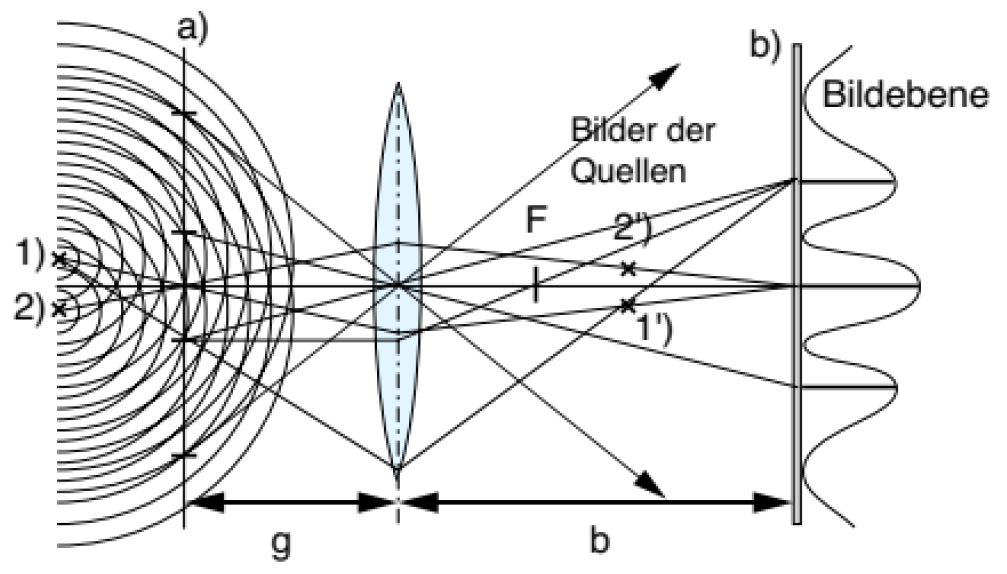
\includegraphics[scale=0.8]{Bilder/Fresnel.png} 
\end{center}
\vspace*{-0.5cm}
\caption[Anordnung der Fresnel'schen Beobachtungsart]{\textbf{Anordnung der Fresnel'schen Beobachtungsart}: Die Wellen der Quellen (1, 2) treffen auf ein Objekt (z.B Spalt) im Nahfeld (a). Die Kugelwellen interferieren dann. Über eine Linse wird das so entstehende Interferenzmuster an einen Schirm (b) \glqq projiziert\grqq\; \cite{Angaben2011}.}
\label{fig:Fresnel}
\end{figure}
\newpage

\subsection{Frauenhofer'sche Beobachtungsart}
\label{subsec:frauenhofBeobachtungsart}
Ein Schirm wird in die Brennebene einer Linse gebracht, welches das Interferenzmuster darauf abbildet. Das somit resultierende Interferenzmuster ist hier nicht von der Lage der Linse zur Quelle abhängig. In der Abbildung \ref{fig:Frauenhofer} zu erkennen.\\
\begin{figure}[h]
\begin{center}
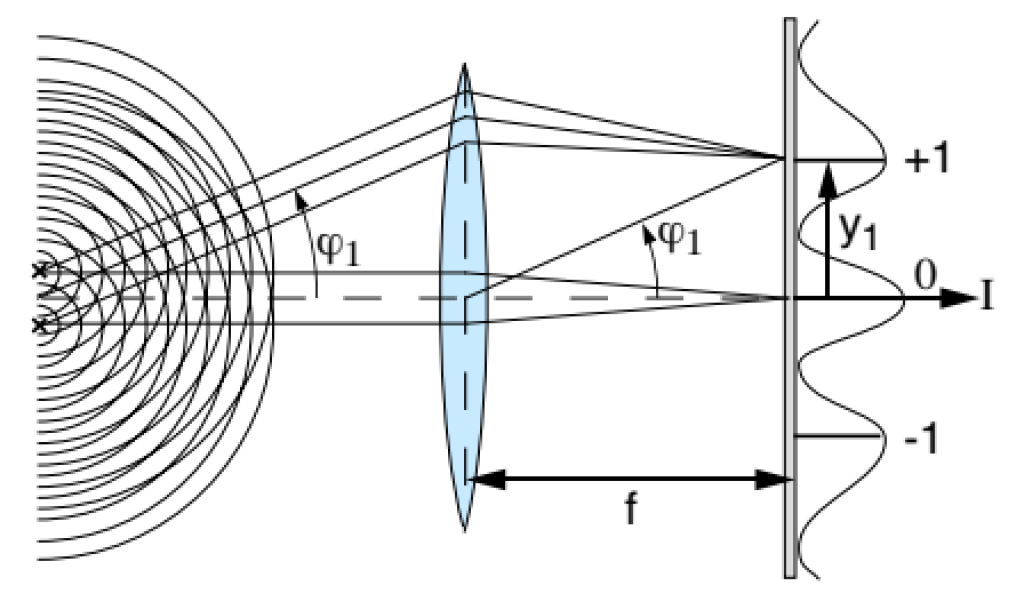
\includegraphics[scale=0.8]{Bilder/Frauenhofer.png}
\end{center}
\caption[Anordnung der Frauenhofer'schen Beobachtungsart]{\textbf{Anordnung der Frauenhofer'schen Beobachtungsart}: Das Interferenzmuster der Interferierenden Wellen wird über eine Linse im Fernfeld auf ein Schirm gegeben. Der Schirm steht in der Brennebene mit dem Abstand der Brennweite f der Linse. Das Interferenzmuster ist so unabhängig von der Linsenposition gegenüber dem Objekt \cite{Angaben2011}.}
\label{fig:Frauenhofer}
\end{figure}

Für die Beugung der Frauenhofer’sche Beobachtungsart gilt folgende Formel \ref{eq:1} \cite{Angaben2011}.\\
%FORMEL1 
\begin{equation}
a_{m}=f\cdot\tan\left( \arcsin\left[ \frac{m\cdot\lambda}{d}\right] \right) 
\label{eq:1}
\end{equation}
$a_{m}$ entspricht der Distanz des Maximums zur Mitte des Interferenzmusters. f der Brennweite. m ist repräsentativ für die Ordnungszahl. $\lambda$ steht für die Wellenlänge des He-Ne-Laserlichts (rot).\\

\subsection{Beugung am Spalt und Antispalt}
\label{subsec:beugspalt}
Beugung am Einzelspalt erzeugt im Fernfeld ein Interferenzmuster, bei welchem sich helle (Maximas) und dunkle (Minimas) Bereiche abwechseln. Die hellen Bereiche sind in der Mitte am hellsten und nach aussen gehend nimmt die Intensität ab. \cite{Angaben2011}.\\

\subsection{Beugung am Loch}
\label{subsec:beugloch}
Bei einer Lochblende wird als Interferenzmuster konzentrisch angelgte Ringe, Maxima und Minima abwechselnd auf dem Schirm beobachtet.\cite{Angaben2011}.\\[0.5cm]
Für die Auswertung bei der Beugung am Loch muss die Ordnungszahl der obigen Formel \ref{eq:1} angepasst werden, da es sich hier um Kreise handelt. Die neue Konstante, welche sich anstelle der Ordnungszahl einfügt, lässt sich gemäss folgender Formel \ref{eq:2} berechnen:
%FORMEL2
\begin{equation}
m_{i}=\frac{J_{1,i}}{\pi}
\label{eq:2}
\end{equation}

\subsubsection{Kreiskoeffizienten für Beugung am Loch}
Die ersten 9 Konstanten (m$_{i}$) werden für diese Arbeit nach der Formel \ref{eq:2} berechnet und unten dargestellt:\\[0.5cm]

\begin{tabular}[h]{ccc}
\centering
Koeffizientennummer & J$_{1,i}$ & m$_{i}$ \\ 
\hline 
1 & 3.832 & 1.220 \\  
2 & 7.016 & 2.233 \\  
3 & 10.173 & 3.238 \\ 
4 & 13.324 & 4.241 \\ 
5 & 16.471 & 5.243 \\ 
6 & 19.616 & 6.244 \\  
7 & 22.760 & 7.245 \\ 
8 & 25.904 & 8.245 \\ 
9 & 29.047 & 9.246 \\ 
\label{table:Koeff}
\end{tabular} 

\subsection{Beugung am Strichgitter}
\label{subsec:beugstrichgitter}
Bei der Beugung am Strichgitter ergibt sich ein Interferenzmuster, bei dem Lichtpunkte entlang der Horizontalen auftreten. Diese Lichtpunkte entstehen durch konstruktive Interferenz an diesen Stellen \cite{Angaben2011}.\\

\chapter{Durchführung}
% =================================================================
\thispagestyle{fancy}
% =================================================================
\section{Versuchsanordnung}
Auf einer Zeiss-Schiene wird das Ganze aufgebaut, auf der die Beugungsobjekte sowie die Linse für die Frauenhofer’sche Beobachtungsart fixiert werden können. Bei jedem Objekt wird erst die direkte Beobachtungsart (jene ohne Linse), anschließend die Frauenhofer’sche Beobachtungsart (jene mit Linse) angewendet. Die zwei Beobachtungsarten werden im Kapitel \nameref{chap:resultateDiskussion} dann mit der Wertvorgabe verglichen.
\\[0.5cm]
Als Lichtquelle steht ein He-Ne-Laser ($\lambda$ = 632.8 nm) zur Verfügung. Mit einem Doppelmeter werden die Distanzen auf der Zeiss-Schiene gemessen. Die Maximas, resp. die Minimas mit Hilfe der Messeinrichtung hinten an der Mattscheibe.\\
\begin{figure}[h]
\begin{center}
\includegraphics[width=\textwidth]{Bilder/Versuchsaufbau.png}
\end{center}
\caption[Versuchsaufbau]{\textbf{Versuchsaufbau}: Zwischen dem He-Ne-Laser und der Mattscheibe mit Messeinrichtung werden die Objekte im Objekthalter befestigt, sowie die Linse mit dem Abstand der Brennweite zur Mattscheibe eingerichtet \cite{TechnikFHNW2014}.}
\label{fig:Versuchsaufbau}
\end{figure}

\noindent
Geräte:
\begin{description}
\item[-]
He-Ne-Laser (rot, 632.8 $\cdot10^{-9}$m)
\item[-]
Doppelmeter (Annahme Abweichung: $s_{f}$ = 1$\cdot10^{-3}$m)
\item[-]
Messeinrichtung (Annahme Abweichung: $s_{a{m}}$= 1$\cdot10^{-3}$m)
\end{description}
\newpage

\section{Messvorgang / Messmethoden}
\subsection{Beugung am Spalt und Antispalt}
Hier werden zwei verschiedene Spalte und zwei verschiedene Antispalte nacheinander auf der Zeiss-Schiene montiert und der Abstand der Beugungsmaximas/minimas zum Mittelpunkt hinten auf der Mattscheibe abgelesen. Anschliessend wird die Spaltendicke d mittels Regression mit QTI-Plot bestimmt. Es werden beide Beobachtungsarten für die Messreihen verwendet.
\subsection{Beugung am Loch}
Es werden zwei verschiedene Löcher nacheinander auf der Zeiss-Schiene montiert und der Abstand der Beugungsminima zum Mittelpunkt bestimmt. Dabei wird dann der Lochdurchmesser des Loches bestimmt. Es werden beide Beobachtungsarten für die Messreihen verwendet.
\subsection{Beugung am Strichgitter}
Es werden zwei verschiedene Strichgitter nacheinander auf der Zeiss-Schiene montiert und der Abstand der Beugungsmaxima zum Mittelpunkt bestimmt. Der Gitterlinienabstand wird dann anschließend bestimmt. Es werden beide Beobachtungsarten für die Messreihen verwendet.
\section{Versuchsobjekte}
\begin{tabular}{|l|l|l|}
\toprule
Objekt & Abmessung & Abweichung $s_{d}$ \\ 
\toprule
Spalt 1& $200\cdot10^{-6}m$ & $\pm4\cdot10^{-6}m$\\ 
Spalt 2& $150\cdot10^{-6}m$ & $\pm4\cdot10^{-6}m$ \\ 
Antispalt 1& $530\cdot10^{-6}m$ & $\pm5\cdot10^{-6}m$ \\ 
Antispalt 2& $430\cdot10^{-6}m$ & $\pm5\cdot10^{-6}m$ \\ 
Loch 1& $150\cdot10^{-6}m$ & $\pm6\cdot10^{-6}m$ \\ 
Loch 2& $100\cdot10^{-6}m$ & $\pm4\cdot10^{-6}m$ \\ 
Strichgitter 1& $100\frac{lines}{mm}$ & keine Angaben \\ 
Strichgitter 2& $80\frac{lines}{mm}$ & keine Angaben \\ 
\bottomrule
\end{tabular} 

\chapter{Auswertung}
% =================================================================
\thispagestyle{fancy}
% =================================================================

\chapter{Fehlerrechnung}
% =================================================================
\thispagestyle{fancy}
% =================================================================
\section{Statistischer Fehler}
Die Aufsummierung der quadrierten partiellen Ableitungen (nach den fehlerbehafteten Grössen) als Diskriminante unter der Wurzel ergibt den statistischen Fehler.\\
\begin{equation}
s=\sqrt{\left( \frac{\partial d}{\partial f} \cdot s_{f}\right)^{2} +\left( \frac{\partial d}{\partial a_{m}} \cdot s_{a_{m}}\right)^{2}}
\label{eq:p3}
\end{equation}

\section{Systematischer Fehler}
Das einige Element in diesem Versuch, welche eine systematische Fehlerquelle wäre, ist der He-Ne-Laser. Da dieser nach \textit{Leif Physik} \cite{PhysikkeineAngaben} mit den höheren und tieferen Energieniveaus der Helium- und Neonatomen arbeitet, ist dessen Unsicherheit auf die Wellenlänge des roten Lichts vernachlässigbar klein. 
\section{Absoluter Fehler}
Statistischer und systematischer Fehler werden quadriert und als Diskriminante unter der Wurzel aufsummiert. Daraus ergibt sich der absolute Fehler jeder Messung. Da aber der systematische Fehler vernachlässigt wird, wäre der absolute Fehler equivalent zum statistischen Fehler.

\chapter{Resultate und Diskussion}
\label{chap:resultateDiskussion}
% =================================================================
\thispagestyle{fancy}
% =================================================================
Durchlaufend durch diese Arbeit wurden jeweils mittels QTI-Plots die Dicke/Lochdurchmesser mit deren Fehlern gefittet (Siehe Kapitel \ref{chap:auswertung} \textit{\nameref{chap:auswertung}}). Im Anhang unter \textit{\nameref{sec:messresultate}} sind die Werte der benutzten Objekten hinterlegt, mit welchen die gefitteten nun graphisch verglichen werden. Die Werte für die Strichgitter sind hier nicht nochmals aufgeführt, da für jene keine Fehlerrechnung gemacht wurde.\\
\begin{figure}[h]
\centering
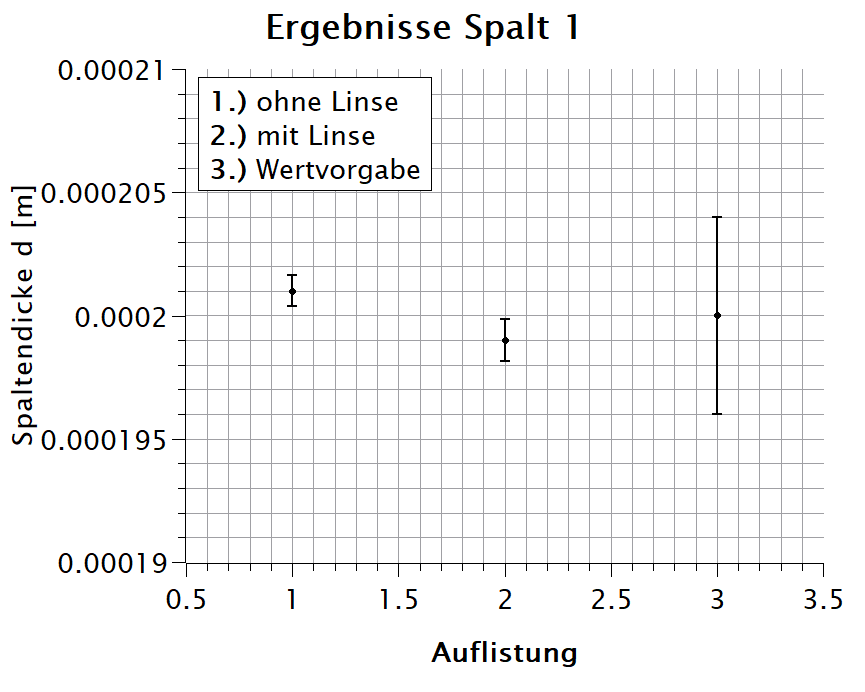
\includegraphics[width=\textwidth]{Bilder/ergebnisse_spalt1.png} 
\caption[Ergebnisse Spalt 1]{Deutlich zu sehen ist, dass die zwei Messreihen (mit und ohne Linse) im Bereich der Wertvorgabe liegen. Der numerische Wert der Wertvorgabe ist in der Abbildung \ref{fig:messresultate1} einzusehen. Somit ist die Spaltendicke verifiziert.}
\label{fig:ergSpalt1}
\end{figure}
\newpage
\begin{figure}
\centering
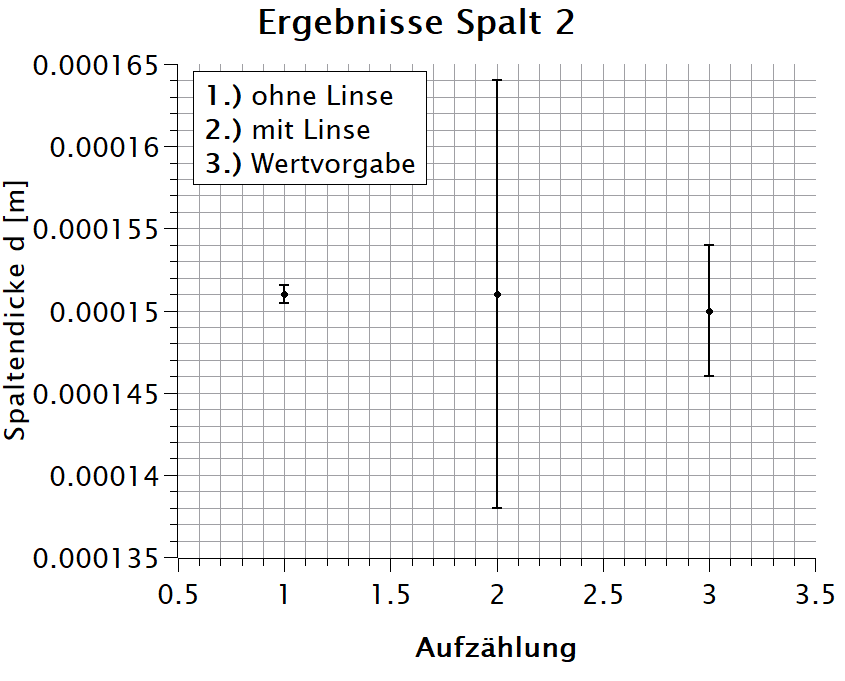
\includegraphics[width=\textwidth]{Bilder/ergebnisse_spalt2.png} 
\caption[Ergebnisse Spalt 2]{Auch hier liegen beide gemessenen Werte innerhalb des Bereiches, welcher von der Wertvorgabe für die Spaltendicke vorgegeben ist. Allerdings ist die Unsicherheit mit der Linse etwas höher, was durch ungenaues Ablesen kausieren könnte. Dennoch ist die Spaltendicke verifiziert.}
\label{fig:ergSpalt2}
\end{figure}
\newpage
\begin{figure}
\centering
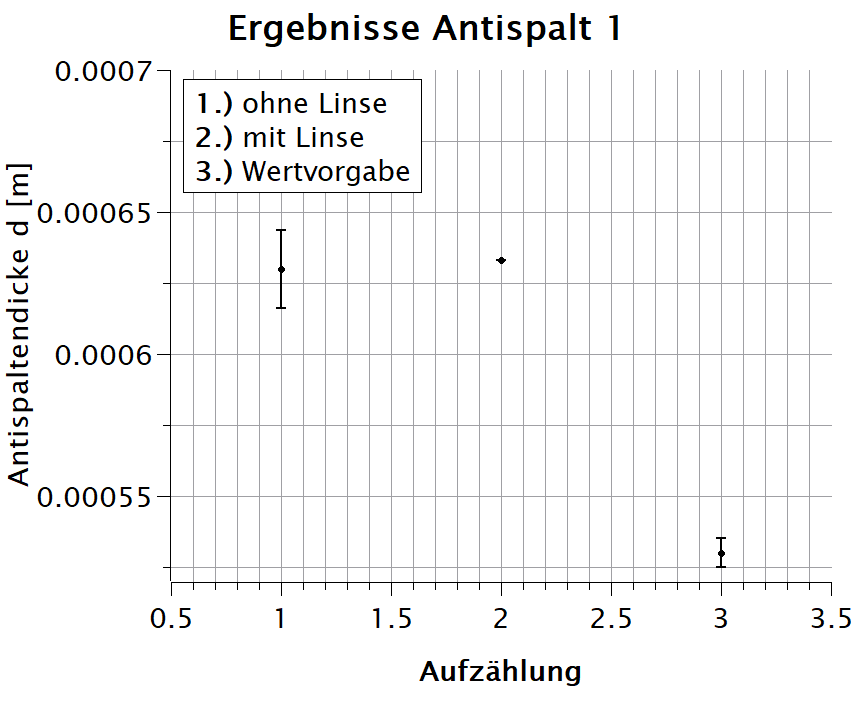
\includegraphics[width=\textwidth]{Bilder/ergebnisse_antispalt1.png} 
\caption[Ergebnisse Antispalt 1]{Hier weicht das Gemessene um ca. 100$\mu$m vom vorgegebenen Wert ab. Dies könnte durch falsches Aufschreiben des Antispalts passiert sein. Denn beide Messreihen liegen sehr nahe beieinander. Zudem sind im Allgemeinen die Messwerte beim Antispalt etwas ungenauer. Es könnte auch auf die falsche Weise gemessen worden sein.}
\label{fig:ergAntispalt1}
\end{figure}
\newpage
\begin{figure}
\centering
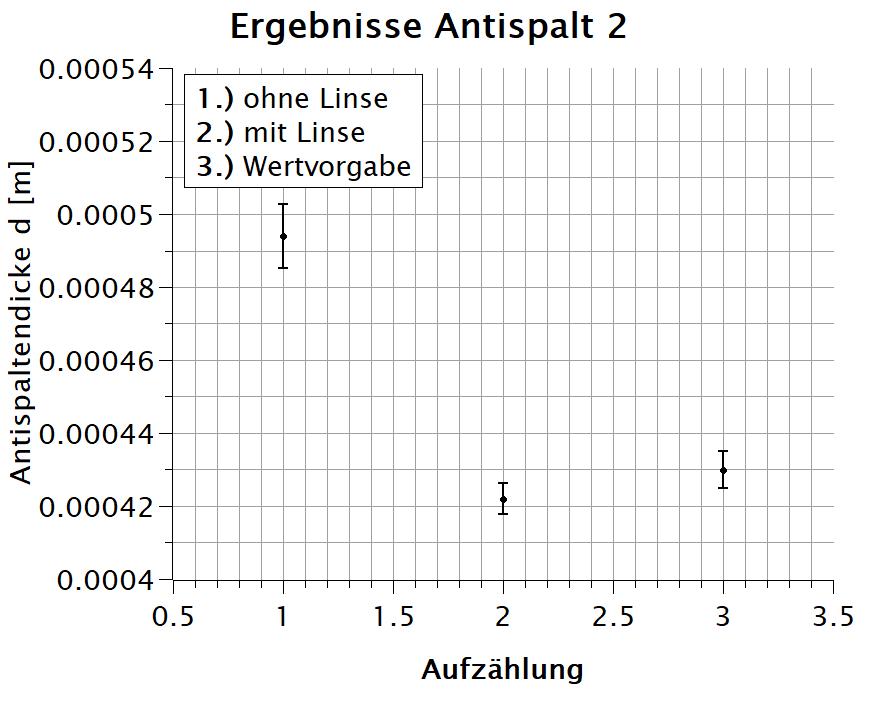
\includegraphics[width=\textwidth]{Bilder/ergebnisse_antispalt2.png} 
\caption[Ergebnisse Antispalt 2]{Die gemessenen Werte liegen ziemlich nahe an der Wertvorgabe beim 2. Antispalt. Besonders die Messreihe mit Linse liegt nur leicht ausserhalb des vorgegebenen Wertes. Auch hier, wie bei Abbildung \ref{fig:ergAntispalt1} könnten die Messwerte genauer sein, wenn die Maximas, anstatt die Minimas gemessen worden wären.}
\label{fig:ergAntispalt2}
\end{figure}
\newpage
\begin{figure}
\centering
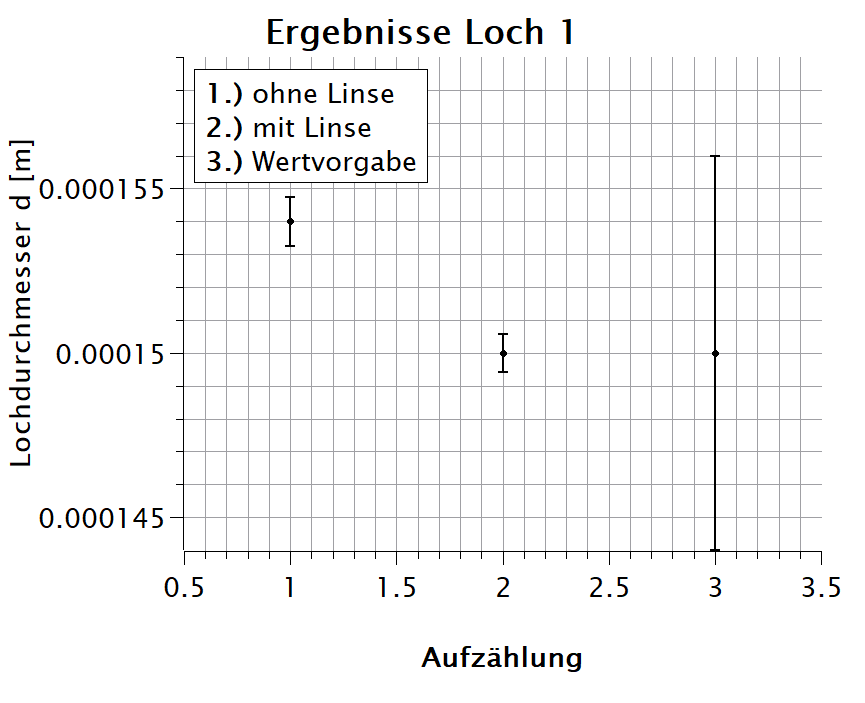
\includegraphics[width=\textwidth]{Bilder/ergebnisse_loch1.png} 
\caption[Ergebnisse Loch 1]{Diese Messreihen mit dem Objekt \textit{Loch} liegen ziemlich genau im vorgegebenem Bereich. Der Lochdurchmesser kann somit als verifiziert betrachtet werden.}
\label{fig:ergLoch1}
\end{figure}
\newpage
\begin{figure}
\centering
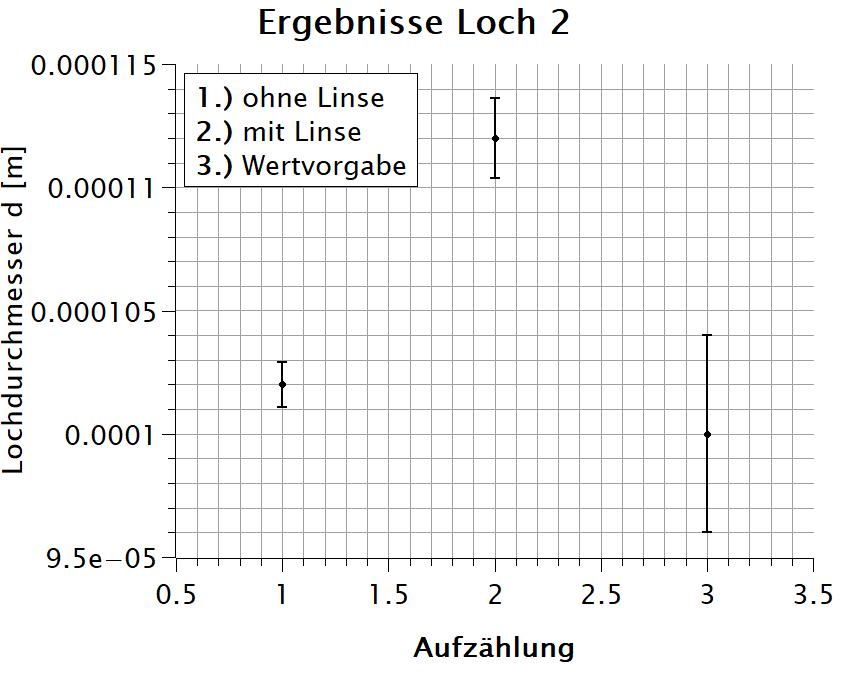
\includegraphics[width=\textwidth]{Bilder/ergebnisse_loch2.png} 
\caption[Ergebnisse Loch 2]{Hier sind die beiden Messreihen etwas zerstreuter als bei der Abbildung \ref{fig:ergLoch1}. Die Messreihe ohne Linse liegt hier deutlich besser im vorgegebenen Bereich als der ohne Linse. Allerdings beträgt die Abweichung nur 6$\mu$m.}
\label{fig:ergLoch2}
\end{figure}
\newpage

\chapter{Plagiatserklärung}
% =================================================================
\thispagestyle{fancy}
% =================================================================
Ich, Andres Minder, der Versuchsleiter in diesem Versuch versichere, dass dieses Laborjournal selbstständig erarbeitet wurde. Alle Quellen und Hilfsmittel aus anderen Werken, die dem Wortlaut oder dem Sinne nach entnommen wurden und zu dieser Arbeit beigetragen haben, sind jeweils kenntlich referenziert.\\
\vfill
\begin{center}
\begin{tabular}{p{5cm}p{1cm}l}
\Large\textbf{Ort, Datum:} & & \Large\textbf{Unterschrift des Versuchsleiters:} \\
\vspace{1cm} & \vspace{1cm} & \vspace{1cm} \\
\centering\Large{Brugg, 15.05.2018} & & \\
\hrulefill & & \hrulefill 
\end{tabular}
\end{center}

\chapter{Verzeichnisse}
% =================================================================
\thispagestyle{fancy}
% =================================================================
\makeatletter
\renewcommand\chapter{\thispagestyle{\chapterpagestyle}%
                    \global\@topnum\z@
                    \@afterindentfalse
                    \secdef\@chapter\@schapter}
\makeatother
\addcontentsline{toc}{section}
{Abbildungsverzeichnis}
\listoffigures
\thispagestyle{fancy}
\newpage

\addcontentsline{toc}{section}{Literaturverzeichnis}
\bibliography{Literaturverzeichnis/lit_o9}
\thispagestyle{fancy}

\chapter*{Anhang}
% =================================================================
\thispagestyle{fancy} \addcontentsline{toc}{chapter}{Anhang}
% =================================================================
\section{Messresultate}
\label{sec:messresultate}
\begin{figure}[h]
\centering
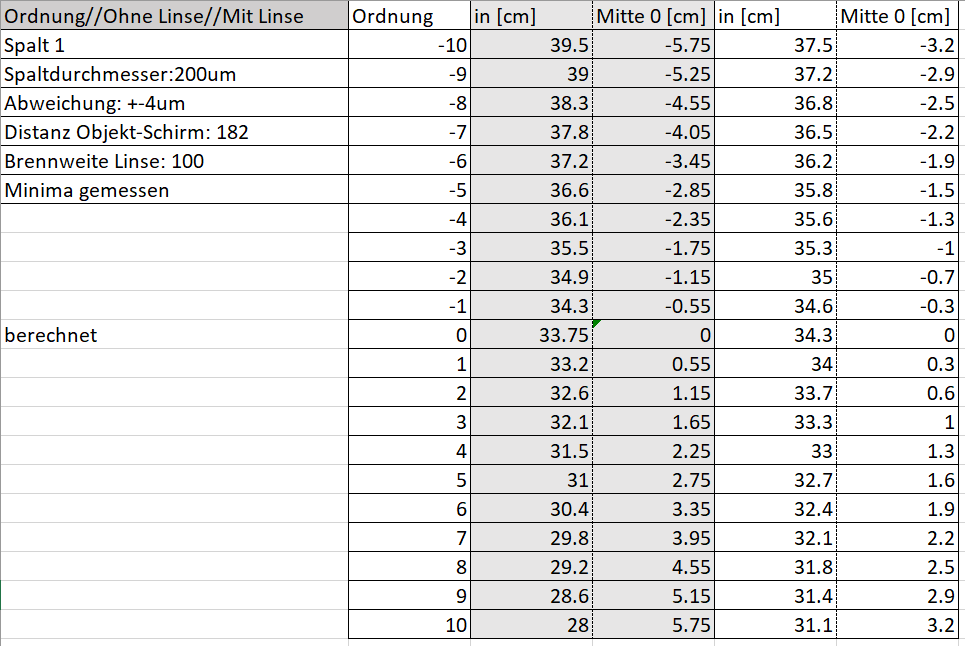
\includegraphics[width=\textwidth]{Bilder/messung1.png} 
\label{fig:messresultate1}
\caption{Messresultate Spalt 1}
\end{figure}
\newpage

\begin{figure}[h]
\centering
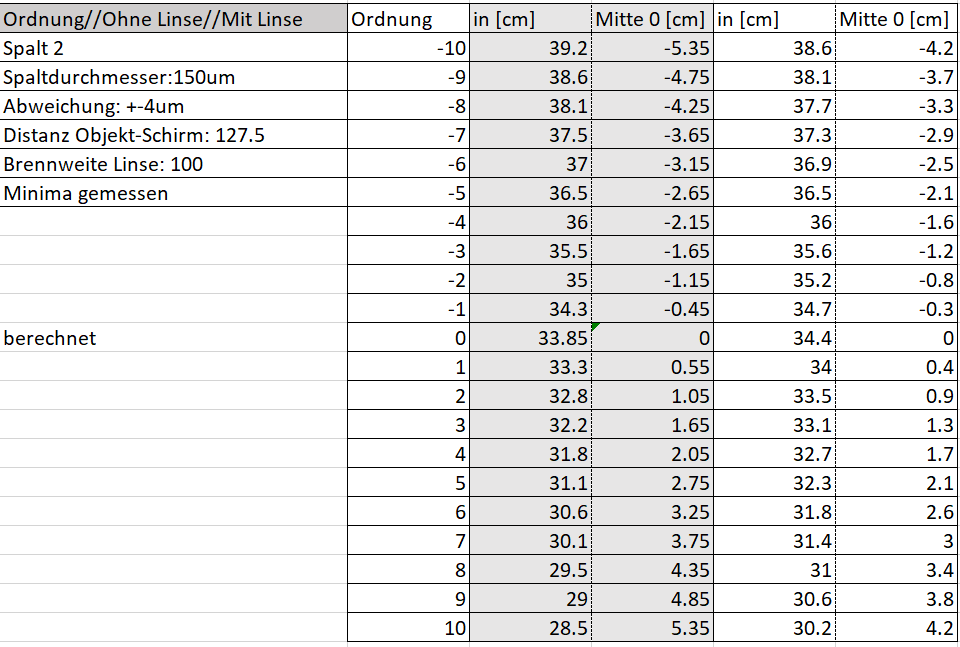
\includegraphics[width=\textwidth]{Bilder/messung2.png} 
\label{fig:messresultate2}
\caption{Messresultate Spalt 2}
\end{figure}
\newpage

\begin{figure}[h]
\centering
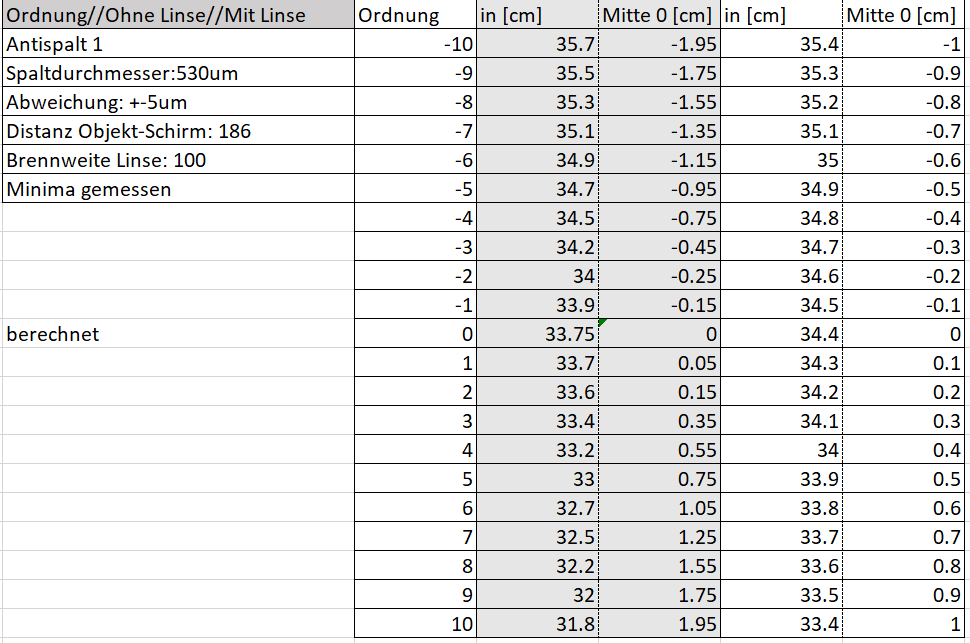
\includegraphics[width=\textwidth]{Bilder/messung3.png} 
\label{fig:messresultate3}
\caption{Messresultate Antispalt 1}
\end{figure}
\newpage

\begin{figure}[h]
\centering
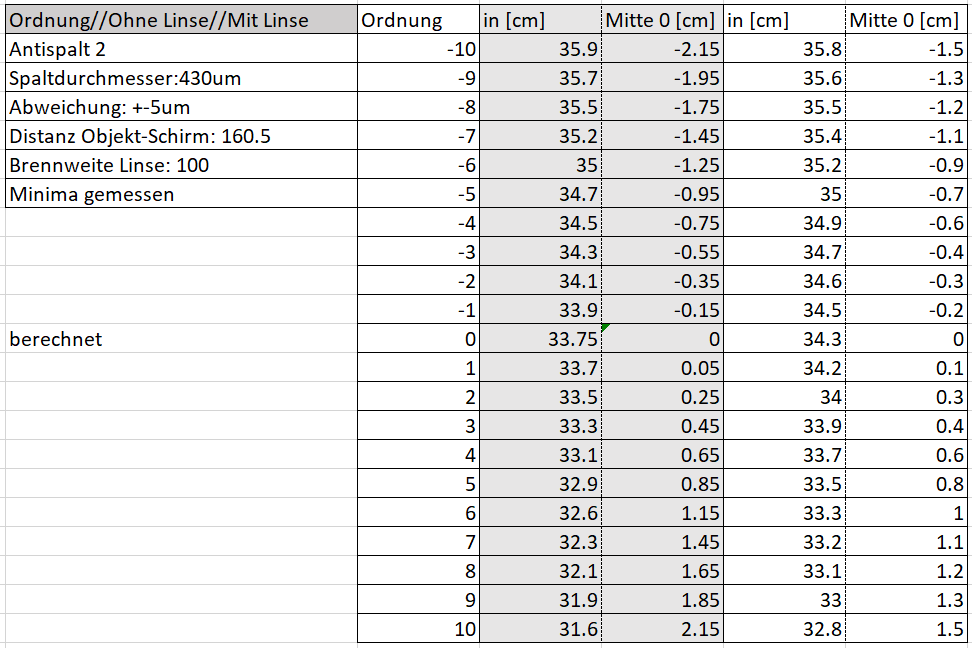
\includegraphics[width=\textwidth]{Bilder/messung4.png} 
\label{fig:messresultate4}
\caption{Messresultate Antispalt 2}
\end{figure}
\newpage

\begin{figure}[h]
\centering
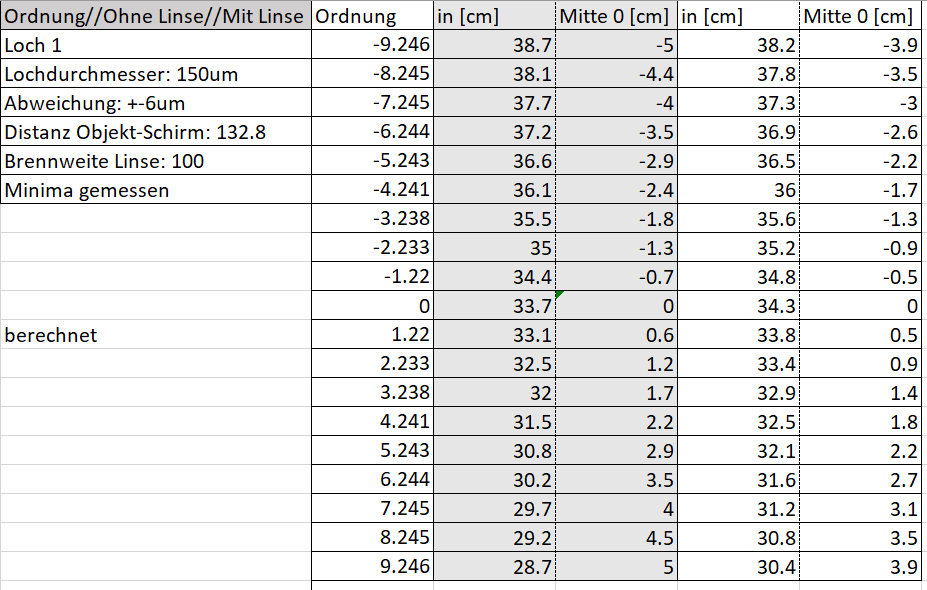
\includegraphics[width=\textwidth]{Bilder/messung5.png} 
\label{fig:messresultate5}
\caption{Messresultate Loch 1}
\end{figure}
\newpage

\begin{figure}[h]
\centering
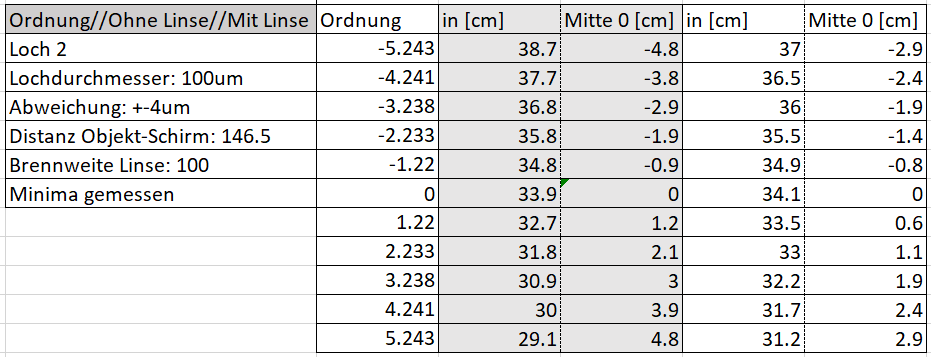
\includegraphics[width=\textwidth]{Bilder/messung6.png} 
\label{fig:messresultate6}
\caption{Messresultate Loch 2}
\end{figure}
\newpage

\begin{figure}[h]
\centering
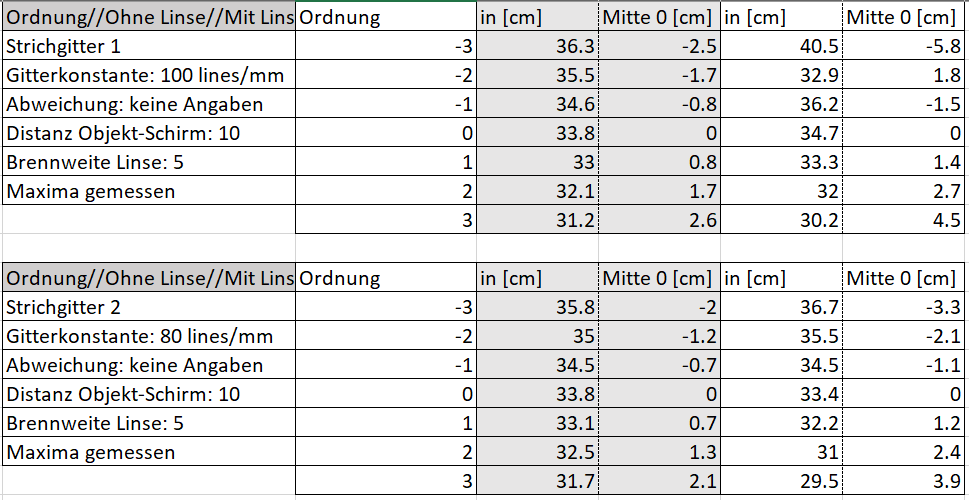
\includegraphics[width=\textwidth]{Bilder/messung7.png} 
\label{fig:messresultate7}
\caption{Messresultate Strichgitter 1\&2}
\end{figure}
\newpage

\section{Beugung am Strichgitter}
\label{sec:BeugungAmStrichgitter}
Auf dem Schirm wurden in diesem Teilversuch die Maximas des Interferenzmusters gemessen und mittels QTI-Plot graphisch dargestellt. Dabei wurden die Gitterlinienabstände mittels der Gleichung \ref{eq:1} ermittelt.

\begin{figure}[h]
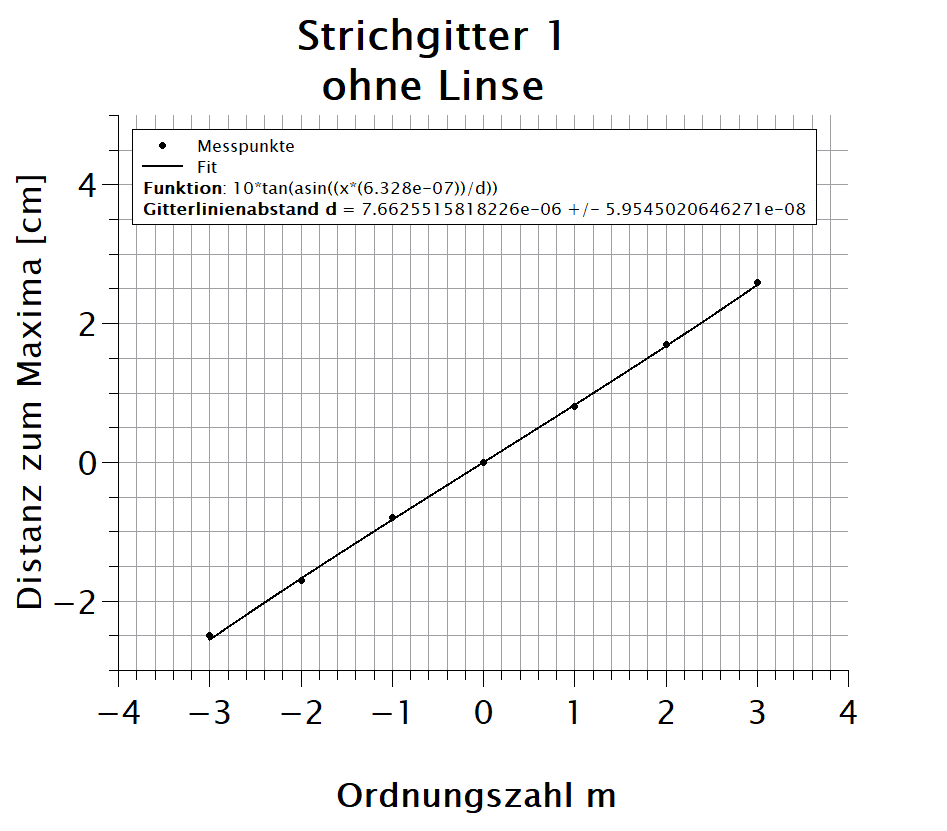
\includegraphics[width=\textwidth]{Bilder/strichgitter1_ohneLinse.png} 
\caption[Strichgitter 1: ohne Linse]{Die Abstände vom Nullpunkt zu den Maximas des Interferenzmusters bei direkter Betrachtung und ohne Linse sind hier graphisch dargestellt. Hier wurde direkt in die Formel \ref{eq:1} der Abstand vom Strichgitter zum Schirm von 10cm eingetragen.}
\label{fig:strichgitter1_ohneLinse}
\end{figure}
\newpage
\begin{figure}[h]
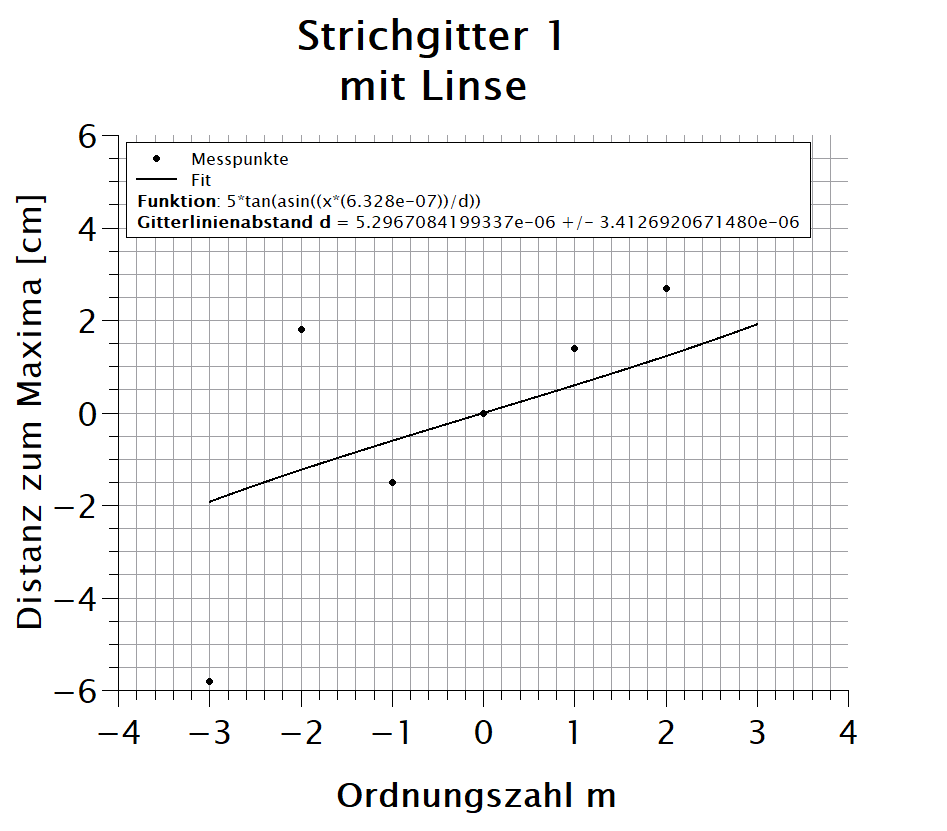
\includegraphics[width=\textwidth]{Bilder/strichgitter1_mitLinse.png} 
\caption[Strichgitter 1: mit Linse]{Die Abstände vom Nullpunkt zu den Maximas des Interferenzmusters bei Frauenhofer'scher Betrachtung und ohne Linse sind hier graphisch dargestellt. Hier wurde direkt in die Formel \ref{eq:1} der Abstand von der Linse zum Schirm von 5cm eingetragen.}
\label{fig:strichgitter1_mitLinse}
\end{figure}
\newpage

\begin{figure}[h]
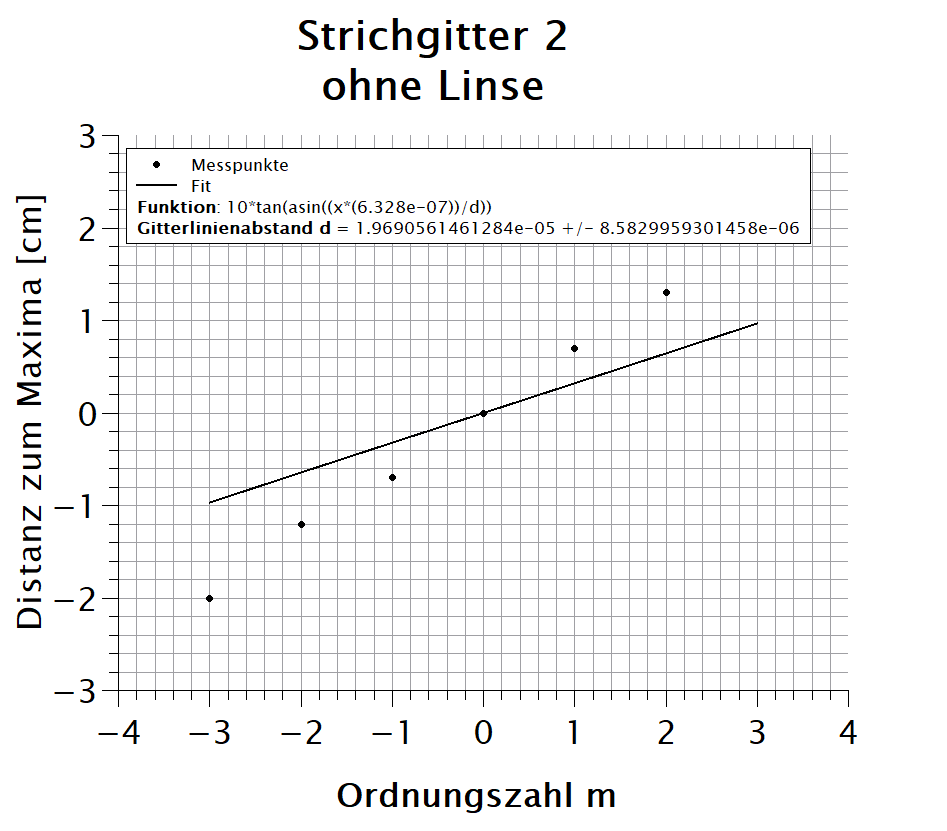
\includegraphics[width=\textwidth]{Bilder/strichgitter2_ohneLinse.png} 
\caption[Strichgitter 2: ohne Linse]{Die Abstände vom Nullpunkt zu den Maximas des Interferenzmusters bei direkter Betrachtung und ohne Linse sind hier graphisch dargestellt. Hier wurde direkt in die Formel \ref{eq:1} der Abstand vom Strichgitter zum Schirm von 10cm eingetragen.}
\label{fig:strichgitter2_ohneLinse}
\end{figure}
\newpage
\begin{figure}[h]
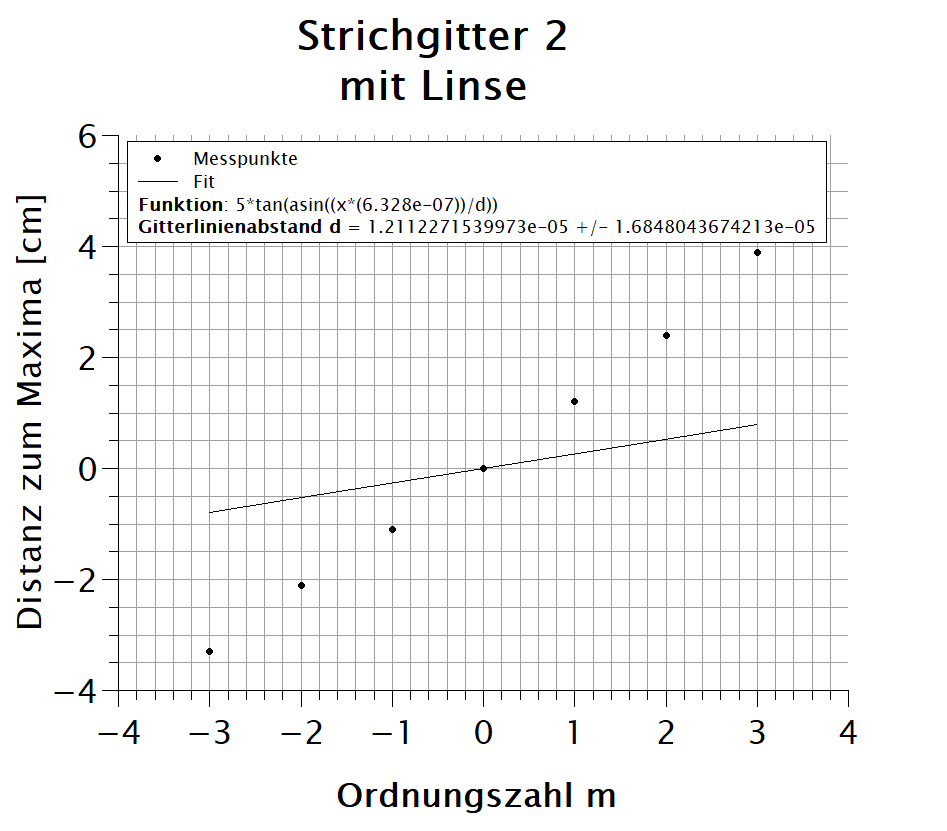
\includegraphics[width=\textwidth]{Bilder/strichgitter2_mitLinse.png} 
\caption[Strichgitter 2: mit Linse]{Die Abstände vom Nullpunkt zu den Maximas des Interferenzmusters bei Frauenhofer'scher Betrachtung und ohne Linse sind hier graphisch dargestellt. Hier wurde direkt in die Formel \ref{eq:1} der Abstand von der Linse zum Schirm von 5cm eingetragen.}
\label{fig:strichgitter1_mitLinse}
\end{figure}
\newpage

\end{document}